\chapter{Coupled Oscillators}

Once we introduce a second (or third, or $N$th) degree of freedom coupled to the first, a single oscillator problem blossoms into a system of coupled ODEs. The organizing principle of this chapter is that every such linear system, no matter how complicated it looks in terms of the physical coordinates $x_1, x_2, \ldots$, can be decomposed into a set of independent \emph{normal modes} --- collective motions in which every part of the system oscillates at a single common frequency and phase. Once the normal modes are in hand, the general motion is nothing more than a superposition of them, and the mathematical problem reduces to that of $N$ uncoupled single oscillators. This chapter develops the machinery in stages: first by brute force on a two-mass example, then by promoting the same calculation to linear algebra, and finally by exploiting symmetry to guess the answer without computing at all.

% ============================================================
\section{Two Coupled Masses}
% ============================================================

Consider two masses $m$ connected in series by three identical springs of spring constant $k$ and natural length $\ell_0$, stretched between two fixed walls a distance $x_w = 3\ell_0$ apart, as in Figure~\ref{fig:two-mass}. Let $x_1$ and $x_2$ denote the positions of the masses measured from the left wall. This is the minimal system that already exhibits all of the qualitative features of a general coupled oscillator, and we will return to it repeatedly for intuition.

\begin{figure}[h]
\centering
\begin{tikzpicture}[
    spring/.style={decorate, decoration={coil, aspect=0.5, segment length=5pt, amplitude=4pt, pre length=4pt, post length=4pt}},
    mass/.style={draw, thick, fill=LightGray, minimum width=1cm, minimum height=1cm}
]
    % walls
    \fill[pattern=north east lines] (-0.35,-0.1) rectangle (0,2.1);
    \draw[thick] (0,-0.1) -- (0,2.1);
    \fill[pattern=north east lines] (11,-0.1) rectangle (11.35,2.1);
    \draw[thick] (11,-0.1) -- (11,2.1);
    % floor
    \draw[thick] (0,0) -- (11,0);
    % springs
    \draw[spring] (0,1) -- (2.5,1);
    \draw[spring] (3.5,1) -- (7.5,1);
    \draw[spring] (8.5,1) -- (11,1);
    % masses
    \node[mass] (m1) at (3,1) {$m$};
    \node[mass] (m2) at (8,1) {$m$};
    % spring labels
    \node at (1.25,1.55) {$k$};
    \node at (5.5,1.55) {$k$};
    \node at (9.75,1.55) {$k$};
    % coordinate labels
    \draw[-{Latex}] (3,-0.5) -- (3.6,-0.5);
    \node at (3,-0.85) {$x_1$};
    \draw[-{Latex}] (8,-0.5) -- (8.6,-0.5);
    \node at (8,-0.85) {$x_2$};
    % wall separation
    \draw[<->] (0,2.4) -- (11,2.4);
    \node at (5.5,2.7) {$x_w = 3\ell_0$};
\end{tikzpicture}
\caption{Two equal masses coupled by three identical springs between fixed walls. The coordinates $x_1$ and $x_2$ measure the mass positions from the left wall.}
\label{fig:two-mass}
\end{figure}

The left spring exerts a force $-k(x_1 - \ell_0)$ on mass~1, while the middle spring is stretched by $(x_2 - x_1 - \ell_0)$ and pulls mass~1 to the right and mass~2 to the left. The right spring is stretched by $(x_w - x_2 - \ell_0)$. Newton's second law gives
\begin{align}
    m\ddot{x}_1 &= k(x_2 - x_1 - \ell_0) - k(x_1 - \ell_0), \\
    m\ddot{x}_2 &= k(x_w - x_2 - \ell_0) - k(x_2 - x_1 - \ell_0).
\end{align}
The constants collapse and we are left with
\begin{equation}
    m\ddot{x}_1 = -2kx_1 + kx_2, \qquad m\ddot{x}_2 = kx_1 - 2kx_2 + kx_w.
\end{equation}

\subsection{Shifting to Equilibrium Coordinates}

The inhomogeneous term $kx_w$ is a nuisance because it prevents us from immediately recognizing the system as a linear one in the sense used for oscillators --- a shift of origin will remove it. Let $x_1' = x_1 - a$ and $x_2' = x_2 - b$ with $a$, $b$ chosen so that $x_1' = x_2' = 0$ is an equilibrium. Substituting demands
\begin{equation}
    -2a + b = 0, \qquad a - 2b = -x_w,
\end{equation}
which yields $a = x_w/3$ and $b = 2x_w/3$ (the masses sit at the natural spring lengths $\ell_0$ and $2\ell_0$ in equilibrium, as one would expect from symmetry). In the shifted variables the equations of motion become homogeneous. Dropping the primes,
\begin{equation}
    \ddot{x}_1 = -\frac{2k}{m}x_1 + \frac{k}{m}x_2, \qquad
    \ddot{x}_2 = \frac{k}{m}x_1 - \frac{2k}{m}x_2.
\end{equation}
Introducing $\omega_0^2 \defeq k/m$, the system reads
\begin{formula}
\begin{equation}
    \ddot{x}_1 = -2\omega_0^2 x_1 + \omega_0^2 x_2, \qquad
    \ddot{x}_2 = \omega_0^2 x_1 - 2\omega_0^2 x_2.
\end{equation}
\end{formula}
The two equations are coupled through the $\omega_0^2 x_j$ terms on the right, which encode the fact that the middle spring feels both displacements at once.

% ============================================================
\section{The Normal-Mode Ansatz}
% ============================================================

The natural way to attack coupled linear ODEs is to look for solutions in which the coupling is invisible --- that is, solutions in which the two masses conspire to move together in such a way that the ratio of their displacements never changes in time. Guided by intuition from the single oscillator, we guess a solution in which \emph{both} masses oscillate at a common frequency $\omega$:
\begin{equation}
    x_1(t) = A_1 e^{i\omega t}, \qquad x_2(t) = A_2 e^{i\omega t}.
\end{equation}
Then $\ddot{x}_j = -\omega^2 A_j e^{i\omega t}$. Substituting and cancelling the exponential factor,
\begin{align}
    -\omega^2 A_1 &= -2\omega_0^2 A_1 + \omega_0^2 A_2, \\
    -\omega^2 A_2 &= \omega_0^2 A_1 - 2\omega_0^2 A_2.
\end{align}
Define the amplitude ratio $r \defeq A_2/A_1$. The first equation gives $-\omega^2 = -2\omega_0^2 + \omega_0^2 r$; the second, divided by $A_1$, gives $-\omega^2 r = \omega_0^2 - 2\omega_0^2 r$. Solving for $\omega^2$ from each and equating leads to $r^2 = 1$, so $r = \pm 1$. Substituting back:
\begin{formula}
\begin{equation}
    \omega_a = \omega_0 = \sqrt{k/m}, \qquad \omega_b = \sqrt{3}\,\omega_0 = \sqrt{3k/m}.
\end{equation}
\end{formula}

\subsection{Interpreting the Frequencies}

The algebra has handed us two frequencies with essentially no physical labor, and it is worth pausing to understand each one before proceeding.

\begin{fact}[Two mode shapes]
The mode with $\omega = \omega_0$ has $r = +1$: the masses move \emph{in phase} with equal amplitude. The middle spring is never stretched or compressed, and each mass sees only its outer spring --- hence $\omega = \sqrt{k/m}$.

The mode with $\omega = \sqrt{3}\,\omega_0$ has $r = -1$: the masses move \emph{antiphase}. The midpoint of the middle spring stays fixed, so each mass effectively sees its outer spring plus half of a middle spring of doubled stiffness $2k$, giving effective spring constant $k + 2k = 3k$ and $\omega = \sqrt{3k/m}$.
\end{fact}

The two mode shapes are sketched in Figure~\ref{fig:normal-modes}. The physical picture generalizes: whenever a symmetric coupled system is decomposed into modes, one mode uses the coupling maximally and one avoids it entirely, and the two frequencies are pushed apart in exact proportion to how strongly the coupling participates.

\begin{figure}[h]
\centering
\begin{tikzpicture}[
    spring/.style={decorate, decoration={coil, aspect=0.5, segment length=4pt, amplitude=3pt, pre length=3pt, post length=3pt}},
    mass/.style={draw, thick, fill=LightGray, minimum width=0.8cm, minimum height=0.8cm},
    disp/.style={-{Latex}, thick, ForestGreen}
]
    % --- symmetric (in-phase) mode, top row ---
    \begin{scope}[yshift=2.6cm]
        \draw[thick] (0,-0.55) -- (0,0.55);
        \draw[thick] (8,-0.55) -- (8,0.55);
        \draw[spring] (0,0) -- (2.1,0);
        \draw[spring] (2.9,0) -- (5.1,0);
        \draw[spring] (5.9,0) -- (8,0);
        \node[mass] (a1) at (2.5,0) {};
        \node[mass] (a2) at (5.5,0) {};
        \draw[disp] (2.5,0) -- ++(0.9,0);
        \draw[disp] (5.5,0) -- ++(0.9,0);
        \node[align=left, anchor=west] at (8.6,0) {$r=+1$,\ \ $\omega_a=\omega_0$\\ in phase};
    \end{scope}
    % --- antisymmetric (antiphase) mode, bottom row ---
    \begin{scope}
        \draw[thick] (0,-0.55) -- (0,0.55);
        \draw[thick] (8,-0.55) -- (8,0.55);
        \draw[spring] (0,0) -- (2.1,0);
        \draw[spring] (2.9,0) -- (5.1,0);
        \draw[spring] (5.9,0) -- (8,0);
        \node[mass] (b1) at (2.5,0) {};
        \node[mass] (b2) at (5.5,0) {};
        \draw[disp] (2.5,0) -- ++(0.9,0);
        \draw[disp] (5.5,0) -- ++(-0.9,0);
        \node[align=left, anchor=west] at (8.6,0) {$r=-1$,\ \ $\omega_b=\sqrt{3}\,\omega_0$\\ antiphase};
    \end{scope}
\end{tikzpicture}
\caption{The two normal modes of the two-mass system. In the symmetric mode (top) both masses move in phase and the middle spring is never stretched; in the antisymmetric mode (bottom) they move antiphase and the middle spring provides extra restoring force, raising the frequency.}
\label{fig:normal-modes}
\end{figure}

\begin{definition}[Normal mode]
A \emph{normal mode} of a linear system is a solution in which every degree of freedom oscillates at the \emph{same frequency} and with a \emph{fixed relative phase}. The corresponding pattern of amplitudes is called the mode shape.
\end{definition}

Since the equations are linear, any linear combination of normal-mode solutions is also a solution. The general motion is a superposition of the four independent normal-mode solutions:
\begin{align}
    x_1(t) &= C e^{i\omega_0 t} + D e^{-i\omega_0 t} + E e^{i\sqrt{3}\omega_0 t} + F e^{-i\sqrt{3}\omega_0 t}, \\
    x_2(t) &= C e^{i\omega_0 t} + D e^{-i\omega_0 t} - E e^{i\sqrt{3}\omega_0 t} - F e^{-i\sqrt{3}\omega_0 t}.
\end{align}
Grouping conjugate pairs and taking the real part gives
\begin{equation}
    x_1(t) = C\cos(\omega_0 t + \varphi_a) + D\cos(\sqrt{3}\omega_0 t + \varphi_b),
\end{equation}
\begin{equation}
    x_2(t) = C\cos(\omega_0 t + \varphi_a) - D\cos(\sqrt{3}\omega_0 t + \varphi_b),
\end{equation}
with four constants $C, D, \varphi_a, \varphi_b$ fixed by four initial conditions $x_1(0), \dot{x}_1(0), x_2(0), \dot{x}_2(0)$. The counting is right: two second-order ODEs give four constants of integration.

% ============================================================
\section{The Matrix Formulation}
% ============================================================

Solving simultaneous equations for the ratio $r$ becomes hopeless with more than two masses, and the calculation quickly becomes opaque even for two if the coupling is unsymmetric. The clean method is linear algebra, which turns the entire problem into an eigenvalue computation. Write $\vect{x} = (x_1, x_2)^T$ and cast the equations of motion as
\begin{equation}
    \ddot{\vect{x}} = P\vect{x}, \qquad
    P = \begin{pmatrix} -2\omega_0^2 & \omega_0^2 \\ \omega_0^2 & -2\omega_0^2 \end{pmatrix}.
\end{equation}
Assume a solution $\vect{x}(t) = \operatorname{Re}\{\vect{A}\, e^{i(\omega t + \varphi)}\}$. Then $\ddot{\vect{x}} = -\omega^2 \vect{x}$, and the equation of motion becomes
\begin{equation}
    -\omega^2 \vect{x} = P \vect{x} \quad \Longrightarrow \quad (P + \omega^2 I)\vect{A} = 0.
\end{equation}
Since the time-dependent factor never vanishes, we need the amplitude vector $\vect{A}$ to lie in the null space of $P + \omega^2 I$. Nontrivial solutions require
\begin{formula}
\begin{equation}
    \det(P + \omega^2 I) = 0.
\end{equation}
\end{formula}
This is the characteristic equation, and its roots $\omega^2$ are the squared normal-mode frequencies; the associated null vectors $\vect{A}$ are the mode shapes. The whole task of finding normal modes is thus equivalent to diagonalizing a single matrix.

\subsection{Applying the Machinery}

For our two-mass system,
\begin{equation}
    \det(P + \omega^2 I) = \det\!\begin{pmatrix} -2\omega_0^2 + \omega^2 & \omega_0^2 \\ \omega_0^2 & -2\omega_0^2 + \omega^2 \end{pmatrix}
    = (-2\omega_0^2 + \omega^2)^2 - \omega_0^4 = 0.
\end{equation}
Thus $-2\omega_0^2 + \omega^2 = \pm\omega_0^2$, giving $\omega^2 = 3\omega_0^2$ or $\omega^2 = \omega_0^2$ --- the same two frequencies as before, reassuringly obtained with a fraction of the algebra.

To find the mode shapes, substitute each $\omega^2$ back. For $\omega_a^2 = \omega_0^2$:
\begin{equation}
    (P + \omega_a^2 I) \vect{A}_a =
    \begin{pmatrix} -\omega_0^2 & \omega_0^2 \\ \omega_0^2 & -\omega_0^2 \end{pmatrix} \vect{A}_a = 0
    \;\Longrightarrow\; \vect{A}_a = C_a \begin{pmatrix} 1 \\ 1 \end{pmatrix}.
\end{equation}
For $\omega_b^2 = 3\omega_0^2$:
\begin{equation}
    (P + \omega_b^2 I) \vect{A}_b =
    \begin{pmatrix} \omega_0^2 & \omega_0^2 \\ \omega_0^2 & \omega_0^2 \end{pmatrix} \vect{A}_b = 0
    \;\Longrightarrow\; \vect{A}_b = C_b \begin{pmatrix} 1 \\ -1 \end{pmatrix}.
\end{equation}
The full solution is the sum
\begin{equation}
    \vect{x}(t) = \vect{A}_a \cos(\omega_a t + \varphi_a) + \vect{A}_b \cos(\omega_b t + \varphi_b),
\end{equation}
with four free constants $C_a, C_b, \varphi_a, \varphi_b$.

The real utility of the matrix method appears when the two masses or the two springs are not equal --- the algebra of the ratio $r$ becomes messy but the determinant remains a routine calculation.

\begin{example}[Hanging masses on unequal springs]
Two masses $m_1 = 4$ and $m_2 = 12$ hang from the ceiling on a chain of springs: an upper spring $k_C = 24$ from ceiling to $m_1$, a middle spring $k_B = 60$ from $m_1$ to $m_2$, and a lower spring $k_A = 72$ hanging below $m_2$ (in some consistent units). Let $y_1, y_2$ be vertical displacements from equilibrium; gravity drops out because the equilibrium already balances it.

Writing Newton's law for each mass and collecting terms,
\begin{equation}
    \ddot{y}_1 = -\frac{k_B + k_C}{m_1} y_1 + \frac{k_B}{m_1} y_2, \qquad
    \ddot{y}_2 = \frac{k_B}{m_2} y_1 - \frac{k_B + k_A}{m_2} y_2.
\end{equation}
Introduce the shorthand $\omega_0^2 = (k_B+k_C)/m_1$, $\omega_1^2 = k_B/m_2$, $\omega_2^2 = k_B/m_1$, $\omega_3^2 = (k_B+k_A)/m_2$. The characteristic equation $\det(P + \omega^2 I) = 0$ becomes
\begin{equation}
    (\omega_0^2 - \omega^2)(\omega_3^2 - \omega^2) - \omega_1^2 \omega_2^2 = 0,
\end{equation}
a quadratic in $\omega^2$ with roots
\begin{equation}
    \omega^2 = \tfrac{1}{2}\!\left[(\omega_0^2 + \omega_3^2) \pm \sqrt{(\omega_0^2 - \omega_3^2)^2 + 4\omega_1^2 \omega_2^2}\right].
\end{equation}
With the numbers above, $\omega_0^2 + \omega_3^2 = 84/4 + 132/12 = 32.5$ and the determinant of the coupling matrix gives $\omega_0^2 \omega_3^2 - \omega_1^2 \omega_2^2 = 166.5$, so
\begin{equation}
    \omega^2 = \frac{32.5 \pm \sqrt{32.5^2 - 4(166.5)}}{2} \;\Longrightarrow\; \omega \approx 5.11,\ 2.52.
\end{equation}
The mode shapes are found by plugging each $\omega^2$ back into $(P + \omega^2 I)\vect{A} = 0$; numerically one obtains $\vect{A}_1 \propto (-2.93, 1)^T$ and $\vect{A}_2 \propto (1.03, 1)^T$. The heavier mass barely participates in the high-frequency mode, as one would expect physically.
\end{example}

% ============================================================
\section{Initial Conditions and Beats}
% ============================================================

\begin{example}[Pluck one mass, hold the other at rest]
Suppose $x_1(0) = x_0$, $x_2(0) = 0$, $\dot{x}_1(0) = \dot{x}_2(0) = 0$. Zero initial velocities force $\varphi_a = \varphi_b = 0$. Then $x_1(0) = C_a + C_b = x_0$ and $x_2(0) = C_a - C_b = 0$, giving $C_a = C_b = x_0/2$. Therefore
\begin{equation}
    x_1(t) = \frac{x_0}{2}\bigl[\cos(\omega_0 t) + \cos(\sqrt{3}\omega_0 t)\bigr], \quad
    x_2(t) = \frac{x_0}{2}\bigl[\cos(\omega_0 t) - \cos(\sqrt{3}\omega_0 t)\bigr].
\end{equation}
Applying the sum-to-product identities
\begin{equation}
    \cos\alpha + \cos\beta = 2\cos\!\left(\frac{\alpha+\beta}{2}\right)\cos\!\left(\frac{\alpha-\beta}{2}\right),
\end{equation}
\begin{equation}
    \cos\alpha - \cos\beta = -2\sin\!\left(\frac{\alpha+\beta}{2}\right)\sin\!\left(\frac{\alpha-\beta}{2}\right),
\end{equation}
we obtain the beat form
\begin{equation}
    x_1(t) = x_0 \cos\!\left(\tfrac{\sqrt{3}+1}{2}\omega_0 t\right) \cos\!\left(\tfrac{\sqrt{3}-1}{2}\omega_0 t\right),
\end{equation}
\begin{equation}
    x_2(t) = x_0 \sin\!\left(\tfrac{\sqrt{3}+1}{2}\omega_0 t\right) \sin\!\left(\tfrac{\sqrt{3}-1}{2}\omega_0 t\right).
\end{equation}
The fast carrier at $\frac{\sqrt{3}+1}{2}\omega_0$ is modulated by the slow envelope at $\frac{\sqrt{3}-1}{2}\omega_0$, and energy sloshes back and forth between the two masses (Figure~\ref{fig:beats}).
\end{example}

\begin{figure}[h]
\centering
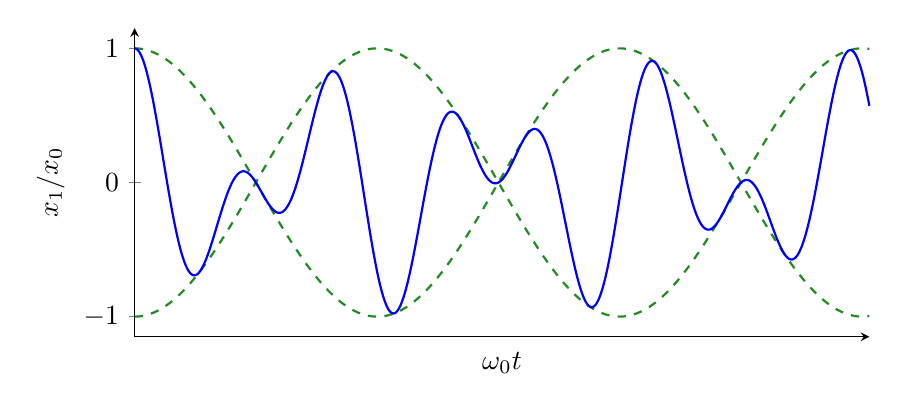
\begin{tikzpicture}
\begin{axis}[
    width=0.9\textwidth, height=5.5cm,
    xlabel={$\omega_0 t$}, ylabel={$x_1/x_0$},
    xmin=0, xmax=26, ymin=-1.15, ymax=1.15,
    axis lines=left,
    xtick=\empty, ytick={-1,0,1},
    enlargelimits=false,
    clip=false
]
    % slow envelope
    \addplot[ForestGreen, dashed, thick, samples=300, domain=0:26]
        {cos(deg(0.36603*x))};
    \addplot[ForestGreen, dashed, thick, samples=300, domain=0:26]
        {-cos(deg(0.36603*x))};
    % beating displacement of mass 1
    \addplot[blue, thick, samples=600, domain=0:26]
        {cos(deg(1.36603*x))*cos(deg(0.36603*x))};
\end{axis}
\end{tikzpicture}
\caption{Beats in the displacement $x_1(t)$ when mass~1 is plucked and mass~2 held at rest. A fast carrier oscillation (solid) is bounded by a slowly varying envelope (dashed); each time the envelope pinches to zero, the oscillation energy has been transferred to the other mass.}
\label{fig:beats}
\end{figure}

\subsection{Energy in Normal Modes vs. Arbitrary Excitations}

The beats example makes vivid a distinction that is worth articulating: only pure normal-mode initial conditions produce simple harmonic motion of the individual masses. Any other initial condition excites more than one mode, and the interference between them produces the beat pattern in each coordinate.

\begin{fact}[Normal mode versus arbitrary excitation]
When the system is set in motion in a pure normal mode, the amplitude ratio is constant, the energy stored in each mass is constant, and the motion is purely harmonic. When the initial condition mixes modes (as in the pluck above), the amplitude ratio varies in time, energy transfers back and forth between the masses, and the motion is not harmonic.
\end{fact}

% ============================================================
\section{Coupled Pendulums}
% ============================================================

The mass-and-spring system is easy to solve but hard to build; the corresponding tabletop demonstration is a pair of pendulums joined by a soft spring. Consider two identical pendulums, each of length $\ell$ and mass $m$, connected by a spring of constant $k$ that is unstretched when both pendulums hang vertically, as in Figure~\ref{fig:coupled-pendulums}. Let $x_1$, $x_2$ be the horizontal displacements of the bobs.

\begin{figure}[h]
\centering
\begin{tikzpicture}[
    spring/.style={decorate, decoration={coil, aspect=0.5, segment length=4pt, amplitude=3pt, pre length=3pt, post length=3pt}}
]
    % ceiling
    \fill[pattern=north east lines] (-0.5,4) rectangle (5.5,4.35);
    \draw[thick] (-0.5,4) -- (5.5,4);
    % pivots
    \coordinate (p1) at (1.5,4);
    \coordinate (p2) at (3.5,4);
    % displaced bob positions
    \coordinate (b1) at (1.9,0.85);
    \coordinate (b2) at (3.9,0.85);
    % vertical reference lines
    \draw[gray, dashed] (p1) -- (1.5,0.6);
    \draw[gray, dashed] (p2) -- (3.5,0.6);
    % rods
    \draw[thick] (p1) -- (b1);
    \draw[thick] (p2) -- (b2);
    % length labels
    \node[left] at ($(p1)!0.5!(b1)$) {$\ell$};
    \node[left] at ($(p2)!0.5!(b2)$) {$\ell$};
    % angle arcs
    \draw (1.5,3.3) arc (270:287:0.7);
    \node at (1.72,3.35) {\small $\theta_1$};
    \draw (3.5,3.3) arc (270:287:0.7);
    \node at (3.72,3.35) {\small $\theta_2$};
    % bobs
    \fill[LightGray, draw=black, thick] (b1) circle (0.28);
    \fill[LightGray, draw=black, thick] (b2) circle (0.28);
    \node at (b1) {\small $m$};
    \node at (b2) {\small $m$};
    % spring between bobs
    \draw[spring] ($(b1)+(0.28,0)$) -- ($(b2)+(-0.28,0)$);
    \node[above] at ($(b1)!0.5!(b2)+(0,0.15)$) {$k$};
    % displacement markers
    \draw[-{Latex}, thick, ForestGreen] (1.5,0.4) -- (1.9,0.4);
    \node[ForestGreen, below] at (1.7,0.35) {\small $x_1$};
    \draw[-{Latex}, thick, ForestGreen] (3.5,0.4) -- (3.9,0.4);
    \node[ForestGreen, below] at (3.7,0.35) {\small $x_2$};
\end{tikzpicture}
\caption{Two identical pendulums of length $\ell$ coupled by a spring of constant $k$. In the small-angle limit the horizontal displacements $x_1, x_2$ obey coupled linear equations, and the spring is unstretched when both bobs hang vertically.}
\label{fig:coupled-pendulums}
\end{figure}

For pendulum 1, the horizontal component of the tension is $-T_1 \sin\theta_1$. In the small-angle limit, $T_1 \cos\theta_1 = mg$ gives $T_1 \approx mg$, and $\sin\theta_1 \approx x_1/\ell$. The spring pulls to the right with $k(x_2 - x_1)$. Thus
\begin{equation}
    m\ddot{x}_1 = k(x_2 - x_1) - \frac{mg}{\ell} x_1, \qquad
    m\ddot{x}_2 = -k(x_2 - x_1) - \frac{mg}{\ell} x_2.
\end{equation}
Rearranging,
\begin{equation}
    \ddot{x}_1 = -\!\left(\frac{k}{m} + \frac{g}{\ell}\right) x_1 + \frac{k}{m} x_2, \quad
    \ddot{x}_2 = \frac{k}{m} x_1 - \!\left(\frac{k}{m} + \frac{g}{\ell}\right) x_2.
\end{equation}
In matrix form, $\ddot{\vect{x}} = P\vect{x}$ with
\begin{equation}
    P = \begin{pmatrix} -\!\left(\tfrac{k}{m} + \tfrac{g}{\ell}\right) & \tfrac{k}{m} \\[3pt] \tfrac{k}{m} & -\!\left(\tfrac{k}{m} + \tfrac{g}{\ell}\right) \end{pmatrix}.
\end{equation}
Define $\omega_1^2 \defeq k/m + g/\ell$ and $\omega_0^2 \defeq k/m$. Then $(P + \omega^2 I)\vect{A} = 0$ requires
\begin{equation}
    (-\omega_1^2 + \omega^2)^2 - \omega_0^4 = 0
    \;\Longrightarrow\; \omega^2 = \omega_1^2 \pm \omega_0^2.
\end{equation}
The two normal frequencies are therefore
\begin{formula}
\begin{equation}
    \omega_+ = \sqrt{\frac{2k}{m} + \frac{g}{\ell}}, \qquad \omega_- = \sqrt{\frac{g}{\ell}}.
\end{equation}
\end{formula}
The lower frequency corresponds to $\vect{A}_- \propto (1, 1)^T$: both pendulums swing together, the spring is never stretched, and the restoring force is purely gravitational. The higher frequency corresponds to $\vect{A}_+ \propto (1, -1)^T$: they swing antiphase, and the spring provides an additional restoring force $2k$ on top of gravity. The two limits $k \to 0$ (no spring) and $k \to \infty$ (rigid link) are illuminating: in the first, the modes degenerate to a single frequency $\sqrt{g/\ell}$, and in the second, the antisymmetric mode is pushed to infinity, leaving only the rigid-body pendulum mode behind.

\begin{example}[Double pendulum with mass ratio $\alpha$]
Consider a double pendulum whose two rods have equal length $L$, with a bob $m_1$ at the middle joint and a bob $m_2$ at the tip. Write $\alpha = m_2/m_1$. In the small-angle limit, the equations of motion (from balancing tensions and horizontal forces) can be written
\begin{equation}
    \ddot{x}_1 = -(2\alpha+1)\omega_0^2\, x_1 + \alpha \omega_0^2\, x_2, \qquad
    \ddot{x}_2 = \omega_0^2\, x_1 - \omega_0^2\, x_2,
\end{equation}
where $\omega_0^2 = g/L$ and $x_1, x_2$ are horizontal displacements of the two bobs. The characteristic equation is
\begin{equation}
    \bigl[-(2\alpha+1)\omega_0^2 + \omega^2\bigr]\bigl[-\omega_0^2 + \omega^2\bigr] - \alpha \omega_0^4 = 0,
\end{equation}
which after expansion becomes $\tfrac{1}{\alpha+1}\omega^4 - 2\omega_0^2 \omega^2 + \omega_0^4 = 0$, with roots
\begin{equation}
    \omega^2 = \omega_0^2 (\alpha + 1)\!\left(1 \pm \sqrt{\tfrac{\alpha}{\alpha+1}}\right).
\end{equation}
Two limits are instructive. As $\alpha \to \infty$ (a heavy tip bob), $\omega^2 \to \omega_0^2 \cdot 2\alpha$ or $\omega_0^2/2$: one very fast mode dominated by the light upper bob whipping around a nearly-fixed tip, and one slow mode in which the two bobs swing nearly as a rigid pendulum of length $2L$. As $\alpha \to 0$ (a massless tip), both roots collapse to $\omega_0^2$, the frequency of the uncoupled upper pendulum.
\end{example}

% ============================================================
\section{General Framework}
% ============================================================

Everything done so far generalizes verbatim to $N$ degrees of freedom. For a system of $N$ masses with equations of motion
\begin{equation}
    M \ddot{\vect{x}} + K \vect{x} = 0,
\end{equation}
where $M = \operatorname{diag}(m_1, \ldots, m_N)$ is the mass matrix and $K$ is the stiffness matrix, plugging in $\vect{x} = \vect{A} e^{i\omega t}$ yields
\begin{equation}
    (-\omega^2 M + K)\vect{A} = 0 \;\Longleftrightarrow\; (M^{-1} K - \omega^2 I)\vect{A} = 0.
\end{equation}
The eigenvalues of $M^{-1} K$ are the squared normal-mode frequencies, and the eigenvectors are the mode shapes. In principle nothing further is required: hand the matrix to a computer and read off the answer.

\subsection{The Zero-Frequency Mode}

In practice one often knows something about the answer before diagonalizing, and the most common piece of prior information concerns a special zero-frequency mode that appears whenever the system as a whole is free to translate.

\begin{fact}[Uniform translation mode]
Whenever the system experiences no net external restoring force --- i.e., all couplings are internal, obeying Newton's third law $K_{ij} = -K_{ji}$ off-diagonal, with zero row sums --- there is a special normal mode with $\omega = 0$ and $\vect{A} \propto (1, 1, \ldots, 1)^T$: a rigid translation of the whole system.
\end{fact}

To see this, sum all rows of the eigenvalue equation with $\vect{A} = (1, 1, \ldots, 1)^T$:
\begin{equation}
    \sum_{i,j} K_{ij} = \omega^2 \sum_i m_i.
\end{equation}
If the row sums of $K$ vanish (no external force), the left side is zero, forcing $\omega^2 = 0$ since $\sum_i m_i > 0$. In such cases, the free constants for a linear-in-time drift $A + Bt$ must be included in the general solution --- a zero-frequency ``oscillation'' is really uniform motion at constant velocity.

\subsection{Utility of the Zero Mode}

Beyond its physical content, the zero mode is useful as a hand-calculation check.

\begin{fact}[Checking a characteristic polynomial]
The characteristic polynomial of a free system (no external force) has the form
\begin{equation}
    \alpha \omega^{2N} + \beta \omega^{2N-2} + \cdots + \zeta = 0,
\end{equation}
and the constant term $\zeta$ \emph{must} vanish, because $\omega = 0$ is always a root. This provides a strong consistency check on hand calculations.
\end{fact}

% ============================================================
\section{Symmetries and Periodic Systems}
% ============================================================

For highly symmetric systems --- say $N$ identical masses arranged in a ring with identical nearest-neighbor springs --- one can bypass the full diagonalization by exploiting the symmetry directly. The idea is that any linear map commuting with the dynamics must share its eigenvectors, so if we can find a simpler operator that reflects the system's geometric symmetry we can read the modes off from \emph{it} instead.

\begin{definition}[Symmetry matrix]
A matrix $S$ is a \emph{symmetry} of the dynamics if $S$ commutes with $M^{-1} K$. Equivalently, if $\vect{x}' = S \vect{x}$ satisfies the same equations of motion whenever $\vect{x}$ does. Common examples: cyclic permutation of sites in a ring, reflection through a symmetry axis.
\end{definition}

If $S$ commutes with the dynamical matrix, its eigenvectors coincide (up to degeneracy) with the normal modes. For a ring of $N$ identical sites, the symmetry $S_1$ that rotates each site to its neighbor satisfies $S_1^N = I$, so its eigenvalues are $N$th roots of unity:
\begin{equation}
    \lambda^{(n)} = e^{i 2\pi n / N}, \qquad n = 0, 1, \ldots, N-1.
\end{equation}
The corresponding eigenvector components are
\begin{equation}
    B_j^{(n)} = \bigl(\lambda^{(n)}\bigr)^{j-1} = e^{i \frac{2\pi n}{N}(j-1)},
\end{equation}
which we may write as $e^{i k^{(n)} j a}$ with wave number
\begin{equation}
    k^{(n)} = \frac{2\pi n}{N a},
\end{equation}
where $a$ is the lattice spacing. This is the origin of the plane-wave normal modes on a periodic lattice, and it foreshadows the continuum wave equation of the next chapter.

\begin{example}[Ring of six masses]
For $N = 6$, the eigenvalues are $\lambda = 1, e^{i\pi/3}, e^{i 2\pi/3}, e^{i\pi}, e^{i 4\pi/3}, e^{i 5\pi/3}$. Each yields one normal mode with amplitude pattern
\begin{equation}
    \vect{B}^{(n)} = \bigl(1,\, \lambda^{(n)},\, (\lambda^{(n)})^2,\, (\lambda^{(n)})^3,\, (\lambda^{(n)})^4,\, (\lambda^{(n)})^5\bigr)^T.
\end{equation}
The periodic boundary condition $x_{N+1} = x_1$ is automatically enforced by $\lambda^N = 1$.
\end{example}

A caveat lurks in the case of highly symmetric systems: symmetry generally forces frequencies to be degenerate, and in a degenerate eigenspace there is no unique choice of eigenvectors.

\begin{fact}[Independence of eigenvectors]
For the general solution to span all initial conditions, the eigenvectors of the dynamical matrix must be linearly independent. Degenerate eigenvalues are fine so long as their eigenspaces are two- (or higher-) dimensional; when they are not, one must supplement the mode expansion with generalized eigenvectors (algebraic terms $t \cdot e^{i\omega t}$, etc.).
\end{fact}

% ============================================================
\section{Damping and Driven Coupled Systems}
% ============================================================

Real coupled systems are damped and often driven, but nothing fundamentally new happens: because the normal-mode decomposition diagonalises the dynamics, each normal mode acts as an independent damped driven oscillator, with its own resonant frequency $\omega_n$. If a sinusoidal drive at frequency $\omega_d$ is applied, the steady-state response is a superposition of Lorentzian resonances peaked at each $\omega_n$. Between resonances the response can dip nearly to zero (antiresonance); at each $\omega_n$ the response is limited only by the damping. Damping of the form $-b\dot{\ell}$, where $\ell$ is the length of a dashpot connecting two masses, adds an antisymmetric term to the equations of motion analogous to the spring coupling but proportional to relative velocity rather than relative position.
